The latter one is inspired by recent development of coding techniques and explores unsupervised heuristics for MKL\cite{ml/BalcanBV06}\cite{nips/YuZG09}\cite{aistats/ZhuangTH11}. For a given point, we deem its kernel evaluation results with other points as its coding. We enforce such coding scheme can well re-construct the point and coincide with its local geometry. Empirical results supports the effectiveness of the proposed techniques.

%---------------------------
\section{Unsupervised Multiple Kernel Learning}
%---------------------------

Traditional multiple kernel learning (MKL) algorithms are essentially supervised in the sense that the kernel learning task requires class labels of the training data. However, class labels may not always be available prior to the kernel learning task in some real world scenarios, such as a clustering task or some early preprocessing step of a classification task.
In this section, we address a new problem of unsupervised multiple kernel learning (UMKL), which does not require class labels of training data in the multiple kernel learning task. As a kernel essentially defines pairwise similarity between any two examples, our unsupervised kernel learning method mainly follows two intuitive principles: (1) a good kernel should allow every example to be well reconstructed from its localized bases weighted by the kernel values; (2) a good kernel should induce kernel values that are coincided with the local geometry of the data. We propose an efficient iterative algorithm to solve the optimization task of the unsupervised multiple kernel learning. Empirical results on a number of UCI data sets verifies the efficacy of our UMKL algorithm.

In this section, we address a new problem of {\em Unsupervised Multiple Kernel Learning} (UMKL), which aims to determine a linear combination of multiple kernels by learning only from unlabeled data.

The UMKL task is more challenging than traditional MKL tasks as no class labels are available to guide the learning task. In this chapter, we propose to attack the unsupervised multiple kernel learning problem by exploiting two intuitions: (1) a good kernel should allow every example to be well reconstructed from its localized bases weighted by the kernel values; (2) a good kernel should induce kernel values that are coincided with the local geometry of the data. We formulate the problem as an optimization task by combining the above two intuitions and propose an iterative algorithm to efficiently solve the optimization task.

%=================================
\subsection{Problem Formulation}
%=================================

Consider a collection of $n$ training samples $\mathcal D = \{(\x_1, y_1),\ldots,(\x_n, y_n)\}$, where $\x_i\in\mathbb{R}^d$ is the input feature vector
and $y_i$ is the unknown class label of $\x_i$, and a set of $m$ predefined kernel functions $\{k_t(\cdot,\cdot),t=1,\ldots,m\}$. The goal of an Unsupervised Multiple Kernel Learning (UMKL) task is to find an optimal linear combination of the $m$ kernel functions, i.e., $k^*(\cdot,\cdot)\in\k_{conv}$, where $\k_{conv}$ is defined as follows:
\begin{equation}
\k_{conv} \!=\!\Big\{k(\cdot,\cdot) \!=\! \sum_{t=1}^m \mu_t k_t(\cdot,\cdot): \sum_{t=1}^m\mu_t  \!=\! 1,\mu_t \!\geq\! 0\Big\}\label{eqn:convex-mkl}
\end{equation}
Unlike supervised MKL, the key challenge of UMKL is how to seek the optimal kernel $k^*(\cdot,\cdot)$ purely from the unlabeled training data. In other words, we need some principles/intuitions to guide the kernel learning task, which should be independent of class labels.

\if 0 We deem kernel as the prior knowledge of the similarity among data, which should be independent of labels. The motivation here is inspired by \cite{nips/YuZG09}, which consists of two pars:\fi

To attack the challenge, we propose to formulate the unsupervised multiple kernel learning task by exploiting the following two intuitive principles:
\begin{itemize}
\item A good kernel should enable each training instance to be well reconstructed from the localized bases weighted by the kernel values. In other words, for each $\x_i$ we expect the optimal kernel can minimize the approximation error $\|x_i-\sum_jk_{ij}\x_j\|^2$;
\item A good kernel should induce kernel values that are coincided with the local geometry of the training data. This is equivalent to finding the optimal kernel that minimizes the distortion over all training data $\sum_{ij}k_{ij}\|\x_i-\x_j\|^2$.
\end{itemize}

Besides, we also exploit the locality preserving principle, which has been shown effective for many unsupervised dimension reduction and semi-supervised learning tasks.In particular, to infer such a local structure, we introduce a set of local bases for each $\x_i\in\mathcal X$, denoted $\mathcal B_i\subset\mathcal X$, which is used to reconstruct sample $\x_i$ and compute the distortion as well. Combining the above principles, we have the final optimization for UMKL:
\begin{eqnarray}
\min_{k, \mathcal B} \frac{1}{2}\sum_{i=1}^n \bigg\| \x_i - \sum_{\x_j\in\mathcal B_i} k_{ij}\x_j \bigg\|^2 + \gamma_1\sum_{i=1}^n\sum_{\x_j\in\mathcal B_i} k_{ij}\big\| \x_i - \x_j \big\|^2 + \gamma_2\sum_i| \mathcal B_i |
\end{eqnarray}
where both the target kernel $k\in \k_{conv}$ and the local basis set $\mathcal B_i$ are unknown variables to be optimized, $\gamma_1$ controls the trade-off between the coding error and the locality distortion, $\gamma_2$ controls the size of local basis set.

To simplify the formulation, for each $\x_i$, we introduce a vector $\d \in\{0,1\}^n$ to indicate its neighbors, i.e., $\mathcal B_i =\{\x_j: d_j\neq0\}$. As a result, the optimization problem can be re-written in a matrix-based form:
\begin{eqnarray}
\hspace{0cm}&\min_{\bm\mu,\D}& \!\!\!\!\frac{1}{2} \Big\| \X \big(\I \!-\! \K\!\circ\!\D\big) \Big\|^2_F \!+\! \gamma_1\tr\K\!\circ\!\D\!\circ\!\M\big(\1\1^\top\big) + \gamma_2 \| \D \|_{1,1} \label{eqn:obj}\\
\hspace{0cm}&\st& [\K]_{ij}=\sum_{t=1}^m\mu_tk^t(\x_i, \x_j), 1\leq i, j \leq n, \bm\mu^\top\1 = 1, \bm\mu\geq 0, \D\in\{0,1\}^{n\times n} \nonumber,
%\nonumber,\\\hspace{0cm}&&
\end{eqnarray}
where the $i$-th column of $\X$ is the point $\x_i$, matrix $[\M]_{ij} := \x_i^\top\x_i+\x_j^\top\x_j - 2\x_i^\top\x_j$ is the Euclidean distance matrix defined on $\X$, $B\in\n_+$ is the parameter controls the size of $\mathcal B_i$ for each $\x_i$. For the above notations, $\circ$ denotes an element-wise multiplication of two matrices, $\|\cdot\|^2_F$ denotes the Frobenius-norm of a matrix, and $tr$ denotes the trace of a matrix.

The presented formulation essentially treats the kernel evaluation $\bm\kappa_i$ as a local coding coordinate of $\x_i$. With the additional constraint $\bm\kappa^\top\1 = 1$, such a local coding system allows a linear approximation of an target function, guaranteed by\cite{nips/YuZG09}:
\begin{theorem}
Let $(\bm\kappa, \mathcal B)$ be an arbitrary coordinate coding on $\mathbb R^d$. Let $f$ be an $(\alpha, \beta, p)$-Lipschitz smooth function, i.e., $| f(\x) - f(\x')| \leq \alpha \| \x - \x'\|$ and $|f(\x') - f(\x) - \nabla f(\x)^\top(\x' - \x)| \leq \beta\|\x - \x'\|^{1+p}$, $\alpha, \beta>0, p\in(0, 1]$. We have for all $\x\in\mathbb R^d$:
\[
\Big| f(\x) - \sum_{\x_j\in\mathcal B}\kappa(\x_i, \x_j)f(\x_j) \Big| \leq \alpha\| \x - \sum_j\kappa_j\x_j \| + \beta \sum_{\x_j\in\mathcal B}| \kappa(\x_i, \x_j) | \| \x_i - \x_i \|^{1+p}.
\]
\end{theorem}
For practical purpose, we remove the constraint $\bm\kappa^\top\1=1$. Instead, we deem the coding as kernel evaluation result, which is sampled from a predefined set $\mathcal K_{conv}$. Moreover, for each data point $\x_i$, we learn a set of local bases, rather than a global basis set. This allows further locality characterization of the data. Such local bases are also useful for discovering the data topology, which is essential for data embedding tasks.

%=================================
\subsection{Iterative Optimization Algorithm}
%=================================

It is not difficult to see that the optimization task (\ref{eqn:obj}) is essentially a mixed integer programming, which is not easy to solve directly. In our approach, we propose an iterative optimization algorithm by alternatively solving $\bm\mu$ and $\D$, which is in spirit to \cite{icml/TanWT10}.

%++++++++++++++++++++++
\subsubsection{Solving $\bm\mu$ by Fixing $\D$}
%++++++++++++++++++++++

We first solve $\bm\mu$ by assuming the values of $\D$ have been identified. The objective reduces to
\begin{eqnarray}
J(\bm\mu) = \bm\mu^\top\bigg(  \sum_{t=1}^m \sum_{i=1}^n\bm\kappa_{t,i}\bm\kappa_{t,i}^\top\circ\mathbf d_i\mathbf d_i^\top\circ\mathbf P              \bigg)\top\bm\mu + \mathbf u^\top\bm\mu,
\end{eqnarray}
where $[\mathbf u]_t:= \sum_{i=1}^n(\mathbf v\circ\mathbf d_i - 2\mathbf p_i\circ\mathbf d_i)^\top\bm\kappa_{t,i}$, $\mathbf P = \X^\top\X$ is the linear kernel, $\bm\kappa_{t,i} :=[k^t(\x_i,\x_1),\ldots,k^t(\x_i,\x_n)]^\top$ is the $i$-th column of the $t$-th kernel matrix,  $\mathbf p$ and $\mathbf v$ are the columns of $\mathbf P$ and $\M$ corresponding to $\x_i$, separately.

As a result, the original optimization problem (\ref{eqn:obj}) w.r.t. $\bm\mu$ is re-formulated into a quadratic program~\cite{Boyd} which can be solved efficiently with off-the-shelf optimization toolkits.

%++++++++++++++++++++++
\subsubsection{Solving $\D$ by Fixing the Kernel} % Greedily}
%++++++++++++++++++++++

The $i$-th column $\mathbf d_i$ of $\D$ is a binary vector indicating the set of localized bases of sample $\x_i$. Note that the columns of $\D$ are independent of each others, i.e., the solution $\mathbf d_i$ of a specific sample $\x_i$ would not affect the bases of other samples. Therefore, we can solve each column $\mathbf d_i$ of $\D$ separately.

At the beginning, we need to find the local basis set for each training sample. To this end, we adopt sparse coding to initialize $\D$, which is formulated into:
\begin{equation}
J(\mathbf d) = \frac{1}{2}\Big\| \x_i - \sum_{j\neq i}d_j\x_j \Big\|^2_2 + \gamma_2\| \mathbf d \|_1. \label{eqn:sparse-coding}
\end{equation}
Note here we relax the binary indicating vector $\mathbf d$ to continuously valued vector. This is a typical sparse coding problem, which can be solved efficiently by feature-sign algorithm \cite{nips/Lee06}.

Assume the we have learned a kernel with the feature mapping function $\Phi$, i.e., $k_{ij} = \Phi(\x_i)^\top\Phi(\x_j)$. The sparse coding (\ref{eqn:sparse-coding}) can be kernelized as
\begin{eqnarray}
J(\mathbf d) &=& \frac{1}{2}\| \Phi(\x_i) - \sum_{j\neq i}d_j\Phi(\x_j) \|_2^2+\gamma_2\| \mathbf d \|_1 \nonumber\\
&=& \frac{1}{2}\big(k_{ii} + \mathbf d_i^\top\mathbf K\mathbf d_i - 2\mathbf d_i^\top\bm\kappa\big) + \gamma_2\| \mathbf d_i \|_1 \nonumber,
\end{eqnarray}
where $\bm\kappa=[k(\x_i,\x_j)]_j$ abbreviates the $i$-th column of the kernel matrix $\mathbf K$. Besides the relaxation of $\D$, another scheme is to propose some greedy algorithm to tackle the original mixed integer programming problem. To this end, we formulate (\ref{eqn:obj}) w.r.t. $\mathbf d$ by
\begin{equation}
J(\mathbf d) = \mathbf d^\top\big(\bm\kappa\bm\kappa^\top\circ\mathbf P\big)\mathbf d + \big(\bm\kappa\circ\mathbf v- 2\bm\kappa\circ\mathbf p\big)^\top\mathbf d, \label{eqn:d}
\end{equation}
where the common subscript of $\mathbf d, \bm\kappa, \mathbf p, \mathbf v$ are omitted.

Let $\U$ abbreviate $\bm\kappa\bm\kappa^\top\circ\mathbf P$, and $\v$ abbreviate $\bm\kappa\circ\mathbf v- 2\bm\kappa\circ\mathbf p$. We solve $\mathbf d$ by a greedy algorithm. Initially, we set all the entries of $\mathbf d$ to zero. At each greedy step, we add one sample into the basis set of $\x$, which implies to set one component of $\mathbf d$ to 1. We choose the component as the one which minimizes the increase of $J(\mathbf d)$. This process is iterated until $B$ entries of $\mathbf d$ have been set to 1.

Assuming each dimension of $\x$ is nonnegative, one can show immediately that $J(\mathbf d)$ is a sub-modular function, i.e., $J(\mathbf d^1) + J(\mathbf d^2) \geq J(\mathbf d^1 | \mathbf d^2) + J(\mathbf d^1 \& \mathbf d^2)$, where $|$ and $\&$ are the bit-wise ``or" and ``and" operation. The following theorem guarantees the performance of greedy selection of $\mathbf d$:
\begin{theorem}
Let $\mathbf d^*$ denote the optimal solution of (\ref{eqn:d}), and $\hat{\mathbf d}$ denote the approximation solution found by the greedy algorithm. We have
\[
J(\hat{\mathbf d}) \geq J(\mathbf d^*)(1 - 1/ e),
\]
if $J(\mathbf d)$ satisfies the following conditions: 1) $J(\mathbf d^1)\leq J(\mathbf d^2)$ if $\mathbf d^1\subset \mathbf d^2$; 2) $J(\mathbf d)$ is a submodular function, and 3) $J(\mathbf 0)=0$.
\end{theorem}




%\begin{algorithm}[htp]\label{alg:umkl}
%\caption{UMKL: Unsupervised Multiple Kernel Learning}
%\textbf{Input:} Unlabeled data $\X$, base kernels $\mathcal K_{base} = \{k_1,\ldots,k_m\}$, $\gamma$, $B$; \\
%\textbf{Output:} Kernel weight $\bm\mu$, bases indicator matrix $\D$.\\\vspace{-0.1in}
%\begin{algorithmic}
%[1]\STATE Initialize $[\M]_{ij} = \x_i^\top\x_i + \x_j^\top\x_j - 2\x_i^\top\x_j$, $\bm\mu=\1/m$, $\mathbf P=\X^\top\X$;
%
%\REPEAT
%
%\STATE $\mathbf W = \sum_{t=1}^m \sum_{i=1}^n\bm\kappa_{t,i}\bm\kappa_{t,i}^\top\circ\mathbf d_i\mathbf d_i^\top\circ\mathbf P$;
%
%\STATE $\bm\mu = \argmin_{\bm\mu}\bm\mu^\top\mathbf W\bm\mu + \mathbf u^\top\bm\mu$;
%
%%\STATE $\nabla J =\sum_{i=1}^n\sum_{\x_j\in\mathcal B_i} \Big(k_{ij}\x_j^\top\x_j - \x_i^\top\x_j + \gamma\|\x_i - \x_j\|^2\Big)k_{ij}^t$;
%
%%\STATE $\bm\mu = \bm\mu + \eta\nabla(J)$;
%
%\FOR{each $\x_i$}
%
%\STATE $\U = \bm\kappa\bm\kappa^\top\circ\mathbf P$,$\v = \bm\kappa(\mathbf v - 2\mathbf p)$;
%
%\STATE Set $\mathcal B_i = \emptyset$;
%
%\FOR{$|\mathcal B_i|<B$}
%
%\STATE $\x^* \!=\! \argmin_{\x_j\in\mathcal X\!-\!\mathcal B_i}2\sum_{t:\x_t\in\mathcal B_i}U_{tj}\!+\!U_{jj} \!+\! v_j$;
%
%\STATE $\mathcal B_i=\mathcal B_i\cup\{\x^*\}$;
%
%\ENDFOR
%
%\ENDFOR
%
%\UNTIL{convergence}
%
%\end{algorithmic}
%\end{algorithm}

After kernel learning, the kernel can be used in classification, or other semi-supervised and unsupervised tasks, such as clustering.

%=======================================================
\subsection{Experiments}\label{sec:exp}
%=======================================================

%=================================
\subsubsection{Experimental Testbed and Setup}
%=================================

We evaluate the performance of the proposed UMKL algorithms for binary classification tasks over a testbed of publicly available data sets as shown in Table 1\footnote{http://www.csie.ntu.edu.tw/~cjlin/libsvmtools/datasets/}
\footnote{http://www.fml.tuebingen.mpg.de/Members/raetsch/benchmark}.

\begin{table*}[!thbp] \label{table:dataset}
%\vspace{-0.2in}
\centering\caption{The statistics of the 12 binary-class data sets used in our experiments.}
%\vspace{-0.1in}
\begin{center}
%\begin{footnotesize}
%\scriptsize
\begin{tabular}{l|rrrrrrrrrr}
\hline
Data Set    &Breast  &Diabetes   &Waveform  &Sonar &Liver  &German\\%&Adult&Ionosphere
\hline
\hline
\# instances      &683  &768    &400    &208    &345    &1,000 \\%&1,605&351
\# dimensions &10   &8  &21 &60 &6  &24\\%&123&33
\hline
\hline
Data Set    &Australian  &Thyroid &Heart    &Banana   &Titanic  &FlareSolar\\%&Splice&Ringnorm
\hline
\hline
\# instances      &690    &140    &270    &400    &150    &666   \\%&1,000&400
\# dimensions  &14 &5  &13 &2  &3  &9    \\% &60&20
\hline
\end{tabular}
%\end{footnotesize}
\end{center}
%\vspace{-0.1in}
\end{table*}

Following the settings of previous MKL studies~\cite{nips/XuJKL08}, for each data set, we create the set of base kernels $\k$ as follows: %for MKL as in
(1) Gaussian kernels with 10 different widths ($\{2^{-3},2^{-2},\ldots,2^6\}$) on all features and on each single feature; (2) polynomial kernels of degree 1 to 3 on all features and on each single feature. Each base kernel matrix is normalized to unit trace. The training instances are normalized to be of zero mean and unit variance, and the test instances are also normalized using the same mean and variance of the training data. To get stable results, for each data set, we repeat each algorithm 20 times and compute the average results of the 20 runs.

Specifically, we have compared the following algorithms:
\begin{itemize}
  \item []\hspace{-1cm}{\bf MKL$^{\mathrm{Level}}$}: The convex multiple kernel learning algorithm, that is, the target
         kernel class is $\k_{conv}$ defined in (\ref{eqn:convex-mkl}). We use the
         extended level method \cite{nips/XuJKL08} to learn the kernel;
  \item []\hspace{-1cm}{\bf LpMKL}: The MKL algorithm with $L_p$ norm regularization over
        the kernel weight \cite{nips/KloftBSLMZ09}. We adopt their cutting plane
        algorithm with second order Taylor approximation of $L_p$;
  \item []\hspace{-1cm}{\bf GMKL}: The Generalized MKL algorithm in \cite{icml/VarmaB09}. The target kernel class is the Hadamard product of single Gaussian kernel defined on each dimension;
  \item[]\hspace{-1cm}{\bf KTA}: The Two-stage Kernel Learning by Kernel Target Alignment algorithm in \cite{icml/Cortes09};
  \item[]\hspace{-1cm}{\bf DMKL}: The Deep MKL framework with \#layer equal to 2 proposed by \cite{aistats/ZhuangTH11};
%  \item[]\hspace{-1cm}{\bf UMKL$^{\mathrm{Spa}}$}: The proposed Unsupervised MKL method with sparse coding to solve basis set;
    \item[]\hspace{-1cm}{\bf UMKL$^{\mathrm{Sub}}$}: The proposed Unsupervised MKL method with greedy basis set selection\footnote{We also evaluated UMKL with the sparse coding solution. We found that it almost always slightly worse than the greedy algorithm.};
\end{itemize}

For parameter settings, the regularization parameter $C$ in SVM for all the compared methods is determined by 5-fold cross validation on the training data over the range of $\{10^{-2}, 10^{-1}, \ldots, 10^2\}$. For a fair comparison, the same set of base
kernels was adopted by MKL$^{\mathrm{Level}}$, LpMKL, KTA, DMKL, and UMKL.  For LpMKL, we examine
$p=2,3,4$ and report the best result.

%=================================
\subsubsection{Experiment I:Unsupervised MKL versus Supervised KL}
%=================================

\begin{table*}[!thbp] \label{table:exp1-result}
\vspace{-0.1in} \centering \caption{The evaluation of classification performance by comparing with a number of different algorithms. Each element in the table shows the mean and standard deviation of classification accuracy (\%). The relative ranking of different MKL algorithms on each data is shown in (). The last row shows the average rank score over all data sets achieved by each algorithm. The {\bf bold} element indicates the best performance.}
\begin{center}
%\setlength{\tabcolsep}{4.5pt}
%\setlength{\extrarowheight}{1.5pt}
{\small
\begin{tabular}{l|l|lllll}
\hline
Data Set  &AvgKernel & MKL$^{\mathrm{level}}$
    &LpMKL  &GMKL  &KTA &UMKL$^{\mathrm{Sub}}$\\
\hline
\hline              %SVM                 LevelMKL            LpMKL               GMKL               IKL                                KDL                     DMKL
Breast          &95.5$\pm$1.0      &96.5$\pm$0.8 &96.2$\pm$0.7  &{\bf 97.0$\pm$1.0}  &96.5$\pm$0.8 &{\bf 97.0$\pm$0.6}\\
Diabetes       &65.4$\pm$2.0  &75.8$\pm$2.5  &72.6$\pm$2.5 &66.4$\pm$2.5   &75.2$\pm$3.3 &{\bf 77.1$\pm$2.3}\\
Titanic         &76.2$\pm$4.2     &77.1$\pm$2.9    &77.0$\pm$3.0 &76.7$\pm$3.1       &78.9$\pm$1.2 &{\bf79.2$\pm$2.5}\\
Heart          &75.6$\pm$6.0    &83.0$\pm$2.9   &76.7$\pm$3.8 &77.0$\pm$3.6    &82.0$\pm$1.9 &{\bf 84.7$\pm$2.6}\\
German          &69.5$\pm$1.5   &71.4$\pm$2.8   &{\bf74.3$\pm$1.4} &70.4$\pm$1.6   &72.1$\pm$1.1 &{\bf74.8$\pm$1.8}\\
Australian     &66.7$\pm$5.6  &85.0$\pm$1.5  &84.5$\pm$1.6 &80.0$\pm$2.3 &{\bf 87.2$\pm$0} &86.3$\pm$1.3\\
Banana         &86.1$\pm$2.3     &90.2$\pm$2.0   &87.5$\pm$2.6 &83.4$\pm$2.7 &{\bf 92.1$\pm$1.7} &90.2$\pm$1.9\\
Thyroid        &82.6$\pm$4.4  &92.9$\pm$2.9    &93.1$\pm$2.2 &94.6$\pm$2.1 &{\bf 97.9$\pm$1.3} &91.2$\pm$2.7\\
FlareSolar     &64.8$\pm$1.6 &{\bf67.6$\pm$2.0}   &64.8$\pm$1.8 &65.3$\pm$1.8  &66.7$\pm$2.3  &{\bf67.8$\pm$1.8}\\
Waveform    &73.5$\pm$7.1 &88.2$\pm$1.6   &{\bf 88.9$\pm$2.0} &88.2$\pm$1.8 &88.5$\pm$2.5 &88.4$\pm$2.5\\
Sonar         &59.1$\pm$9.7 &78.3$\pm$3.5&{\bf 84.8$\pm$3.2} &78.8$\pm$4.6 &81.3$\pm$2.9 &81.0$\pm$2.9\\
Liver       &57.6$\pm$2.3       &62.3$\pm$4.5 &{\bf 69.4$\pm$2.9} &63.6$\pm$2.6 &68.7$\pm$1.5 &68.3$\pm$4.3\\
\hline
\end{tabular}
}
\end{center}
\end{table*}

The first experiment is to examine whether the proposed UMKL can produce good results comparing with traditional supervised kernel learning (SKL) algorithms with the same set of training data. For each data set, we randomly sample $50\%$ of all instances as training data, and use the rest as test data. The classification accuracy is shown in Table 2, from which we can draw two observations:

First, UMKL is comparable with supervised kernel learning algorithms. Among the evaluated 12 data sets, UMKL reports 6 best results, which is the largest among all the evaluated methods. None of the compared 4 algorithms, i.e., MKL, LpMKL, GMKL, and KTA, can outperform the proposed UMKL algorithm significantly. The average rank of UMKL is comparable with KTA. These three algorithms are significantly better than MKL and GMKL. This result verifies the efficacy of UMKL clearly. When the half of the data have labels for training, SKL and UMKL, which does not use the label information, produce similar classification accuracy.

Second, among the SKL algorithms, KTA and DMKL yield the best performance. The average rank of DMKL among SKL algorithms is the best, quite similar to KTA.. Traditional MKL cannot result in the best accuracy on any evaluated data sets. The results of KTA on {\em thyroid} are statistically significant better than other SKL methods. In Figure 1 we illustrate the performance of UMKL and KTA with varying fraction of training points.

\begin{figure*}[!t]
\begin{center}
\subfigure[heart]{
\includegraphics[width=2.5in]{figures/heart.eps}
}
\subfigure[breast]{
\includegraphics[width=2.5in]{figures/titanic.eps}
}
\caption{Accuracy of UMKL and KTA with varying \#train/\#test. }
\end{center}
\end{figure*}

%=================================
\subsubsection{Experiment II: Clustering Accuracy of UMKL}
%=================================

\begin{figure*}[!ht]\hspace{-0.1in}
\begin{center}
\subfigure[k-means clustering]{
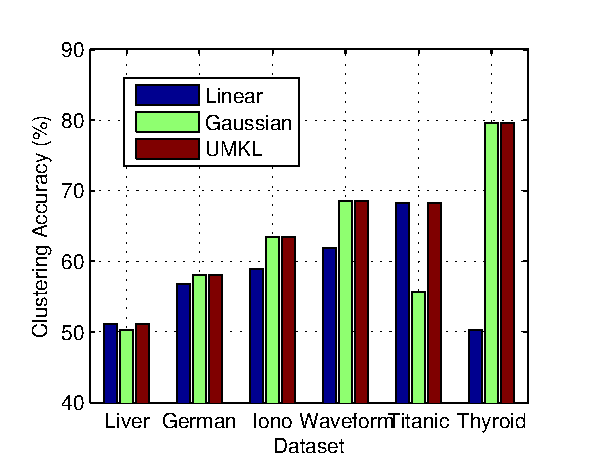
\includegraphics[width=2.5in]{figures/kmeans.eps}%1.51
}
\subfigure[spectral clustering]{
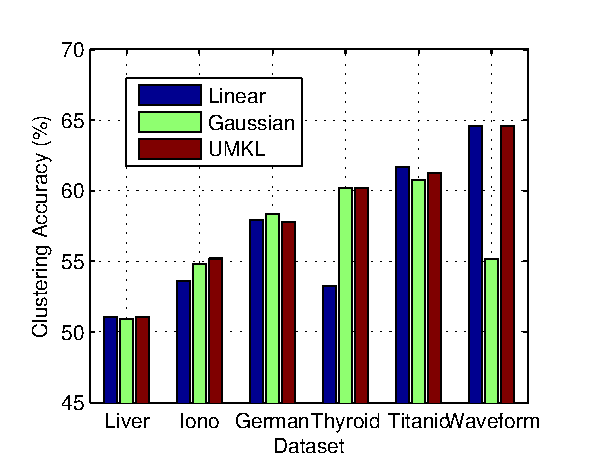
\includegraphics[width=2.5in]{figures/spectral.eps}
}
\caption{The clustering accuracy of linear kernel, Gaussian kernel, the kernel learned by UMKL on 6 benchmark data sets. The parameter $B$ of UMKL is fixed to 10.}
\end{center}
\end{figure*}

The basic motivation of UMKL is to learn a kernel that can reveal the local structure of the data. In this section, we examine whether the kernel learned by UMKL can be better than simple kernels in unsupervised task, specifically, in the k-means and spectral clustering algorithms. We compare UMKL with Gaussian kernel, in which the bandwidth parameter $\sigma$ is set to be the mean square Euclidean distance. The clustering accuracy is defined as in \cite{nips/XingNJR02}:
\[
Accuracy = \sum_{i>j} \frac{ \mathbb I\big\{\mathbb I\{c_i=c_j\}=\mathbb I\{\hat{c}_i=\hat{c}_j\} \big\} } {0.5n(n - 1)},
\]
where $\mathbb I\{\cdot\}$ is the indicator function that outputs 1 when the input is true and 0 otherwise. $c_i$ and $\hat{c}_i$ denote the true cluster membership and the predicated cluster membership of the $i$-th data point.

The clustering accuracy is plotted in Figure 2. Among the 6 evaluated data sets, UMKL can be better than a traditional linear or Gaussian kernel. For the {\em titanic} data set, linear kernel is much better than Gaussian kernel, while for the {\em thyroid} data set Gaussian kernel is better (we take k-means for an example). In advance, end users would not know which kernel is better for the data. UMKL can help find the best kernels. For both {\em titanic} and {\em thyroid}, UMKL yields almost the best performance. But (\ref{eqn:obj}) is not designed for clustering after all. Similar to the case that MKL cannot beat single kernel with cross validation, UMKL cannot produce better kernel for clustering than a properly chosen single kernel.

Referring to our objective function (\ref{eqn:obj}), we seek a kernel that can reconstruct an input point (the first term) and minimize the distortion between kernel evaluation and distance from its nearby neighbors (the second term). Due to this enforcement, the kernel learned by UMKL has a larger chance to preserve the local geometry in the input space than a simple parametric kernel.

%=======================================================
\subsection{Conclusion}\label{sec:con}
%=======================================================

In this section we propose an unsupervised multiple kernel learning (UMKL) algorithm which do not rely on class labels. We deem the kernel evaluation of each sample as its local coding. Then we proposed an efficient iterative algorithm to learn the kernel and the local set of basis simultaneously. Empirical results show that the kernel learned by UMKL is comparable with supervised MKL algorithms. It can also find the data structure effectively such that clustering performance is also guaranteed. We conclude UMKL attractive as in real applications class labels are often expensive to obtain. 